\documentclass[11pt]{article}

\usepackage[margin=1in]{geometry}
\usepackage{amsmath,amssymb,mathtools}
\usepackage{graphicx}
\usepackage{booktabs}
\usepackage{array}
\usepackage{hyperref}
\usepackage{enumitem}
\usepackage{xcolor}
\usepackage{microtype}

\hypersetup{
  colorlinks=true,
  linkcolor=blue!55!black,
  citecolor=blue!55!black,
  urlcolor=blue!55!black
}

\newcommand{\R}{\mathbb{R}}
\newcommand{\N}{\mathcal{N}}
\newcommand{\E}{\mathcal{E}}
\newcommand{\G}{\mathcal{G}}
\newcommand{\one}{\mathbf{1}}
\newcommand{\eps}{\varepsilon}
\newcommand{\dd}{\mathrm{d}}

\title{Data Graph Constructions for Geodesic Distance Approximation}
\author{gflow development note}
\date{Build timestamp: \today}

\begin{document}
\maketitle

\begin{abstract}
This report describes data-to-graph constructions for approximating intrinsic geodesic
distances from finite samples.  The motivating problem is to construct a weighted graph
\(G(X)=(V,E,\ell)\), with \(V=X\), whose shortest-path metric \(d_G\) approximates
geodesic distances on an underlying structured object.  This requires two separate
choices: an edge support that blocks false ambient shortcuts while retaining enough local
connectivity, and edge lengths that represent local travel costs rather than unrelated
similarities.  We compare directed kNN, symmetric kNN, mutual kNN, intersection kNN,
fixed-radius graphs, adaptive-radius graphs, and PHATE's thresholded adaptive affinity
support.  PHATE remains important here, but as an affinity and diffusion construction
whose nonzero support is close to a threshold-inflated symmetric kNN or max-rule
adaptive-radius graph.  We also describe local geodesic pruning, older iKNN-specific
global pruning, component-MST connectivity repair, and practical examples where folds,
branches, near crossings, density changes, and quadratic graph surfaces stress the graph
construction.
\end{abstract}

\section{Introduction}

Many high-dimensional data sets are not well represented by ambient Euclidean distance
alone.  Samples may lie near a nonlinear manifold, a curve network, a branching state
space, a folded surface, a loop, a stratified object, or a noisy tube around one of these
ideal geometries.  In such settings, two observations can be close in \(\R^p\) while far
along the intrinsic object.  This happens across folds, near self-approaches, at crossing
or nearly crossing branches, and in regions where noise fills a small ambient gap.  The
reverse problem also appears: points that are intrinsically adjacent can be separated by
sampling density variation, local curvature, or finite-sample holes.

The purpose of a data graph for geodesic reconstruction is to turn the observed sample
into a finite metric proxy for intrinsic travel.  A good graph allows paths to follow
locally supported data geometry.  A bad graph admits short circuits across unrelated
nearby branches, or disconnects the sample so that finite graph distances become infinite.
The central design tension is therefore local: keep enough edges to follow the object, but
not so many that the graph forgets the difference between ambient proximity and intrinsic
adjacency.

This report grew out of an audit of PHATE's graph construction in \texttt{gflow}.  PHATE
does not build an ordinary k-nearest-neighbor graph.  It first constructs directed adaptive
affinities, thresholds small entries, symmetrizes, and then row-normalizes the resulting
kernel to obtain a diffusion operator.  With the usual PHATE decay and threshold values,
the nonzero undirected support is close to a slightly inflated symmetric kNN support.  That
observation motivates the broader comparison in this report: if the support geometry is
what matters for graph shortest paths, then symmetric kNN, mutual kNN, intersection kNN,
fixed-radius, and adaptive-radius graphs should be studied directly as graph-geodesic
estimators.

\section{The data geodesic reconstruction problem}

Let
\[
  X=\{x_1,\ldots,x_n\}\subset \R^p
\]
be a finite sample from, or near, a structured geometric object \(M\).  When a continuous
target exists, let \(d_M\) denote the intrinsic geodesic distance on \(M\).  For a smooth
Riemannian manifold, for example,
\[
  d_M(x,y)
  =
  \inf_{\gamma(0)=x,\ \gamma(1)=y}
  \int_0^1
  \sqrt{g_{\gamma(t)}(\dot{\gamma}(t),\dot{\gamma}(t))}\,\dd t .
\]
For branching or stratified data, \(d_M\) should be read more generally as the shortest
admissible intrinsic path length on the object being sampled.

A data graph construction maps \(X\) to a weighted undirected graph
\[
  G(X)=(V,E,\ell),
  \qquad
  V=\{1,\ldots,n\},
  \qquad
  \ell_{ij}>0\ \text{for}\ \{i,j\}\in E.
\]
The graph shortest-path distance is
\[
  d_G(i,j)
  =
  \min_{i=v_0,\ldots,v_m=j}
  \sum_{r=0}^{m-1} \ell_{v_r v_{r+1}},
\]
with \(d_G(i,j)=\infty\) when \(i\) and \(j\) lie in different connected components.  The
guiding reconstruction goal is
\[
  d_G(i,j) \approx d_M(x_i,x_j)
  \qquad \text{for sampled pairs } i,j.
\]
In finite simulations one can also compare against a sample-oracle distance
\(d_X^{\mathrm{oracle}}\), which asks how well the reference geodesic can be represented by
paths through the observed sample points.  If \(\gamma_{ij}\) is a reference geodesic and
\((a_0,\ldots,a_m)\) is an ordered set of observed sample points near it, then a typical
sample-oracle target is
\[
  d_X^{\mathrm{oracle}}(i,j)
  =
  \sum_{r=0}^{m-1}
  \|x_{a_{r+1}}-x_{a_r}\|_2 .
\]
The continuum target tests whether the graph recovers the underlying geometry.  The
sample-oracle target tests whether the graph is close to the best route that the finite
observations could plausibly support.

Most graph families in the current \texttt{gflow} benchmark use ambient Euclidean edge
lengths,
\[
  \ell_{ij}=\|x_i-x_j\|_2.
\]
This is a length convention, not an affinity convention.  iKNN can also carry native
intersection-mediated detour lengths, and PHATE produces affinities that must not be
treated as graph lengths without an explicit transformation.

\section{Conventions and terminology}

Let \(D=(d_{ij})\) be a symmetric nonnegative input distance matrix with \(d_{ii}=0\).  In
Euclidean examples,
\[
  d_{ij}=\|x_i-x_j\|_2.
\]
For \(k\in\{1,\ldots,n-1\}\), let \(N_k(i)\) be the \(k\) nearest non-self neighbors of
vertex \(i\), using deterministic tie-breaking when needed.  Define the closed
neighborhood
\[
  \widehat{N}_k(i)=\{i\}\cup N_k(i),
\]
and the local \(k\)-neighbor radius
\[
  \sigma_i=d_{i,(k)}.
\]
When there are no nearest-neighbor ties,
\[
  j\in N_k(i)
  \quad\Longleftrightarrow\quad
  d_{ij}\le \sigma_i.
\]

\begin{center}
\scriptsize
\begin{tabular}{@{}p{0.16\linewidth}p{0.15\linewidth}p{0.41\linewidth}p{0.19\linewidth}@{}}
\toprule
Construction & Primary object & Edge support & Default length or weight \\
\midrule
Directed kNN & directed search graph & \(i\to j \Longleftrightarrow j\in N_k(i)\) & search primitive \\
sKNN/uKNN & undirected graph & \(j\in N_k(i)\) or \(i\in N_k(j)\) & length \(\|x_i-x_j\|_2\) \\
mKNN & undirected graph & \(j\in N_k(i)\) and \(i\in N_k(j)\) & length \(\|x_i-x_j\|_2\) \\
iKNN & undirected graph & \(\widehat{N}_k(i)\cap\widehat{N}_k(j)\ne\varnothing\) & detour or direct length \\
Fixed radius & undirected graph & \(d_{ij}\le \eps\) & length \(\|x_i-x_j\|_2\) \\
Adaptive radius & undirected graph & \(d_{ij}\le c\,h(\sigma_i,\sigma_j)\) & length \(\|x_i-x_j\|_2\) \\
PHATE & affinity/diffusion & \(K_{ij}>0\) after thresholding & affinity, then Markov transition \\
\bottomrule
\end{tabular}
\end{center}

\section{Graph construction families}

\subsection{Directed kNN}

The directed kNN graph is the primitive returned by a nearest-neighbor search:
\[
  i\to j
  \quad\Longleftrightarrow\quad
  j\in N_k(i).
\]
It need not be symmetric.  In graph-geodesic reconstruction, the directed lists are usually
converted into an undirected support before shortest paths are computed.

\subsection{Symmetric kNN}

The symmetric kNN graph, also called the union kNN graph, keeps an undirected edge when at
least one endpoint selects the other:
\[
  \{i,j\}\in E_{\mathrm{sKNN}}
  \quad\Longleftrightarrow\quad
  j\in N_k(i)\ \text{or}\ i\in N_k(j).
\]
In the no-tie case this is equivalent to the max-scale rule
\[
  \{i,j\}\in E_{\mathrm{sKNN}}
  \quad\Longleftrightarrow\quad
  d_{ij}\le \max(\sigma_i,\sigma_j).
\]
This graph is usually better connected than mutual kNN, especially in regions where sample
density changes.  Its cost is that the one-sided OR rule can admit cross-density or
near-fold shortcut edges.

\subsection{Mutual kNN}

The mutual kNN graph keeps only reciprocal neighbor relations:
\[
  \{i,j\}\in E_{\mathrm{mKNN}}
  \quad\Longleftrightarrow\quad
  j\in N_k(i)\ \text{and}\ i\in N_k(j).
\]
Without ties,
\[
  \{i,j\}\in E_{\mathrm{mKNN}}
  \quad\Longleftrightarrow\quad
  d_{ij}\le \min(\sigma_i,\sigma_j).
\]
mKNN is therefore a min-scale adaptive graph.  It is conservative and often useful for
suppressing false local shortcuts, but it can disconnect finite samples at small \(k\) or
across nonuniform density.

\subsection{Intersection kNN}

The intersection kNN graph uses closed neighborhoods:
\[
  \{i,j\}\in E_{\mathrm{iKNN}}
  \quad\Longleftrightarrow\quad
  \widehat{N}_k(i)\cap \widehat{N}_k(j)\ne\varnothing .
\]
This is not equivalent to a direct radius condition on \(d_{ij}\).  Two points can be
connected because both share a third nearby point, even if neither endpoint selects the
other as a direct neighbor.  In \texttt{gflow}, the native iKNN length for edge \(\{i,j\}\)
is an intersection-mediated detour,
\[
  \ell_{ij}^{\mathrm{iKNN}}
  =
  \min_{c\in \widehat{N}_k(i)\cap \widehat{N}_k(j)}
  \left(d_{ic}+d_{jc}\right).
\]
If the intersection contains one of the endpoints, this can equal the direct distance
\(d_{ij}\); otherwise it records a local two-hop detour through a shared neighbor.

\subsection{Fixed-radius graphs}

The fixed-radius graph uses a global distance threshold:
\[
  \{i,j\}\in E_\eps
  \quad\Longleftrightarrow\quad
  d_{ij}\le \eps .
\]
It is the deterministic data-analysis analogue of a random geometric graph when samples
are random and the same \(\eps\) is applied globally.  The algorithm is conceptually simple:
compute candidate pair distances, keep those below \(\eps\), assign local lengths, and
optionally repair connectivity.  The main weakness is density sensitivity.  A radius that
connects sparse regions may over-connect dense or near-fold regions; a radius that blocks
shortcuts in dense regions may disconnect sparse ones.

\subsection{Adaptive-radius graphs}

Adaptive-radius graphs replace the global radius with a local scale.  Let
\[
  \sigma_i=d_{i,(k_{\mathrm{scale}})}.
\]
For radius factor \(c>0\), \texttt{gflow} currently supports
\[
  \{i,j\}\in E_{\mathrm{adapt,max}}
  \quad\Longleftrightarrow\quad
  d_{ij}\le c\,\max(\sigma_i,\sigma_j),
\]
and
\[
  \{i,j\}\in E_{\mathrm{adapt,min}}
  \quad\Longleftrightarrow\quad
  d_{ij}\le c\,\min(\sigma_i,\sigma_j).
\]
With \(c=1\) and matching no-tie conventions, the max rule recovers sKNN support and the
min rule recovers mKNN support.  Values \(c>1\) inflate the adaptive radius; values
\(c<1\) make the graph more conservative.  This family makes explicit that sKNN and mKNN
are not merely neighbor-list tricks, but special cases of local-scale radius rules.

\begin{figure}[htbp]
  \centering
  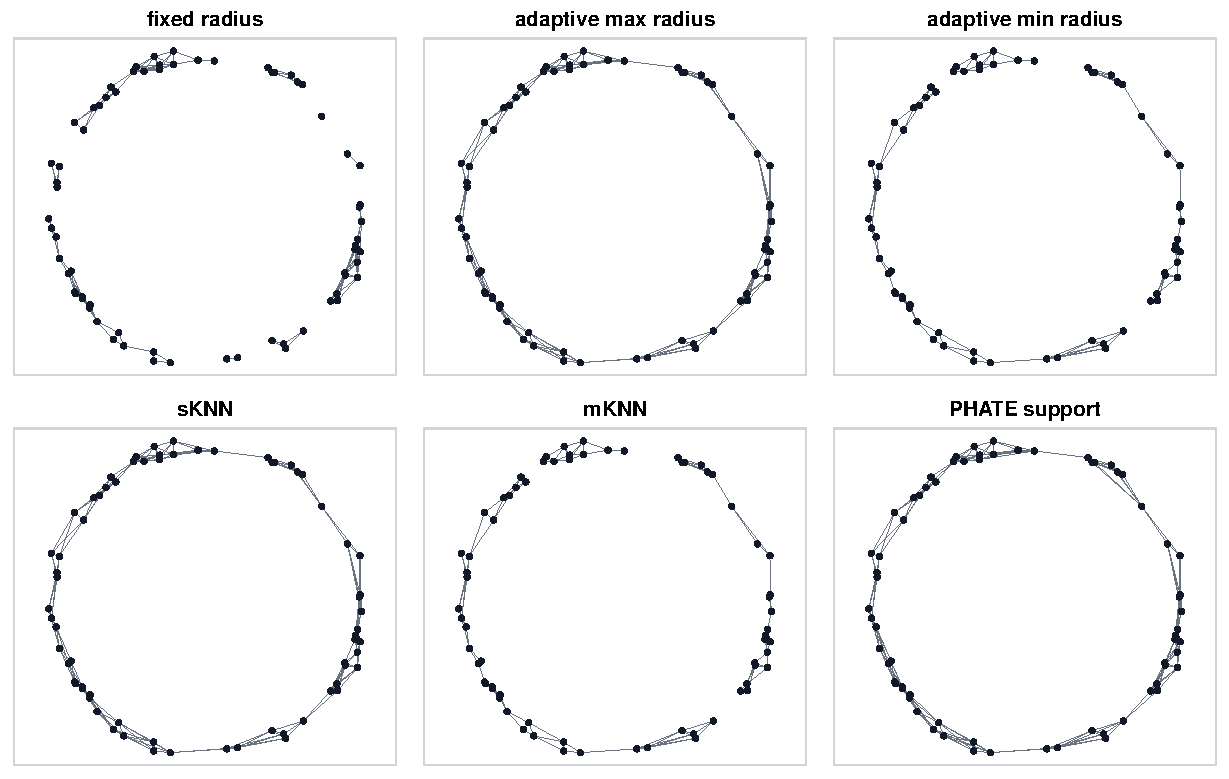
\includegraphics[width=\linewidth]{figures/construction_rules_nonuniform_circle.pdf}
  \caption{Graph construction rules on a nonuniform noisy circle.  Fixed radius uses one
  global scale, adaptive max and sKNN use the larger endpoint scale, adaptive min and mKNN
  use the smaller endpoint scale, and PHATE support is a threshold-inflated adaptive max
  support.}
\end{figure}

\subsection{PHATE adaptive affinity support}

PHATE constructs a directed adaptive affinity rather than a length graph.  With local scale
\(\sigma_i=b\,d_{i,(k)}\), decay \(a>0\), and threshold \(\tau\),
\[
  A_{ij}
  =
  \exp\left[-\left(\frac{d_{ij}}{\sigma_i}\right)^a\right],
  \qquad
  A_{ii}=1,
\]
then small directed affinities are set to zero:
\[
  A_{ij}=0
  \quad\text{if}\quad
  A_{ij}<\tau .
\]
The directed survival condition is
\[
  d_{ij}\le r_\tau\sigma_i,
  \qquad
  r_\tau=(-\log\tau)^{1/a}.
\]
For PHATE's common values \(a=40\) and \(\tau=10^{-4}\),
\[
  r_\tau=(-\log 10^{-4})^{1/40}\approx 1.057.
\]
With additive symmetrization,
\[
  K_{ij}=\frac{A_{ij}+A_{ji}}{2},
\]
the undirected nonzero support is
\[
  \{i,j\}\in E_{\mathrm{PHATE}}
  \quad\Longleftrightarrow\quad
  d_{ij}\le r_\tau\max(\sigma_i,\sigma_j).
\]
This is exactly a max-rule adaptive-radius graph support with local scales
\(\sigma_i\) and radius factor \(r_\tau\).  Thus PHATE's support is close to
sKNN when \(r_\tau\) is close to one.  PHATE then row-normalizes \(K\) to obtain
a Markov transition matrix
\[
  P_{ij}=\frac{K_{ij}}{\sum_{\ell=1}^n K_{i\ell}}.
\]
The matrix \(P\) is useful for diffusion geometry and embedding, but it is not a
graph-geodesic length matrix.  Turning affinities into lengths requires an additional
modeling choice, for example
\[
  \ell_{ij}=-\log(K_{ij}+\eta)
  \quad\text{or}\quad
  \ell_{ij}=K_{ij}^{-1/q},
\]
and those transformations should be treated as separate research questions.

\section{Support relations}

Under common \(D\), common \(k\), no ties, PHATE additive symmetrization, and \(r_\tau\ge 1\),
the direct radius-like supports satisfy
\[
  E_{\mathrm{mKNN}}
  \subseteq
  E_{\mathrm{sKNN}}
  \subseteq
  E_{\mathrm{PHATE}} .
\]
The first inclusion follows from AND implying OR.  The second follows from
\[
  \max(\sigma_i,\sigma_j)\le r_\tau\max(\sigma_i,\sigma_j).
\]
iKNN is different.  It is based on shared closed neighborhoods, not on a direct
radius threshold.  Therefore neither
\[
  E_{\mathrm{iKNN}}\subseteq E_{\mathrm{PHATE}}
  \qquad\text{nor}\qquad
  E_{\mathrm{PHATE}}\subseteq E_{\mathrm{iKNN}}
\]
holds in general.  Empirically, iKNN can be denser than PHATE, but the relationship is not a
simple nesting hierarchy.

\begin{center}
\small
\begin{tabular}{lll}
\toprule
Relationship & Holds under matching no-tie conventions? & Reason \\
\midrule
\(E_{\mathrm{mKNN}}\subseteq E_{\mathrm{sKNN}}\) & yes & reciprocal implies one-sided \\
\(E_{\mathrm{sKNN}}\subseteq E_{\mathrm{PHATE}}\) & yes if \(r_\tau\ge 1\) & threshold inflation \\
\(E_{\mathrm{mKNN}}\subseteq E_{\mathrm{iKNN}}\) & yes for closed iKNN & endpoints are shared \\
\(E_{\mathrm{iKNN}}\subseteq E_{\mathrm{PHATE}}\) & no & shared-neighbor predicate \\
\(E_{\mathrm{PHATE}}\subseteq E_{\mathrm{iKNN}}\) & no & direct adaptive radius predicate \\
\bottomrule
\end{tabular}
\end{center}

\section{Pruning graph supports}

Graph construction often produces edges that are locally redundant or geometrically
suspicious.  Pruning is a post-construction sparsification stage.  It should not be
conflated with the original support rule: a pruned sKNN graph and a native mKNN graph can
have similar edge counts while representing different local decisions.

\subsection{Local geodesic pruning}

Local geodesic pruning is the main cross-family pruning method currently used in
\texttt{gflow}.  Let \(G=(V,E,\ell)\) be a candidate graph.  For an edge \(\{u,v\}\) with
length \(\ell_{uv}\), define a local vertex set \(L(u,v)\).  In the current implementation,
\[
  L(u,v)=\{u,v\}\cup N_{k_{\mathrm{local}}}(u)\cup N_{k_{\mathrm{local}}}(v),
\]
where the local neighborhoods are computed from the ambient sample coordinates.  Temporarily
exclude the edge \(\{u,v\}\) and compute the shortest alternative path from \(u\) to \(v\)
inside the induced local graph:
\[
  d_{L(u,v)\setminus\{uv\}}(u,v)
  =
  \min_{\pi:u\leadsto v,\ \pi\subseteq L(u,v),\ \{u,v\}\notin\pi}
  \sum_{\{a,b\}\in\pi}\ell_{ab}.
\]
For tolerance \(\tau_{\mathrm{prune}}>1\), prune the edge when
\[
  d_{L(u,v)\setminus\{uv\}}(u,v)
  \le
  \tau_{\mathrm{prune}}\,\ell_{uv}.
\]
Edges are processed longest-first.  Intuitively, a direct edge is removed when nearby
retained edges already provide a path that is only slightly longer.  This is spanner-like in
spirit, but it is a pragmatic local data-graph rule rather than a proof-carrying global
spanner construction.

\begin{figure}[htbp]
  \centering
  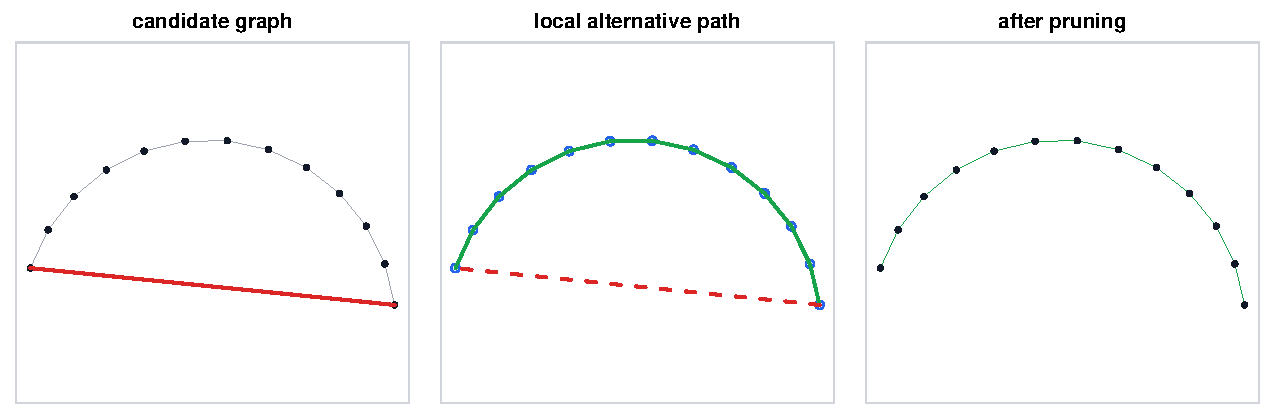
\includegraphics[width=0.95\linewidth]{figures/local_geodesic_pruning_diagram.pdf}
  \caption{Local geodesic pruning.  A long candidate chord is tested against an alternative
  path restricted to a local neighborhood.  If the alternative path length is at most
  \(\tau_{\mathrm{prune}}\ell_{uv}\), the chord is locally redundant and can be removed.}
\end{figure}

\subsection{iKNN global geometric pruning and long-edge pruning}

\texttt{create.single.iknn.graph()} also retains older iKNN-specific global geodesic
pruning.  It considers candidate long edges and removes an edge when the whole current graph
contains an alternative path whose path-to-edge ratio is below a threshold.  In notation,
one tests whether
\[
  \frac{d_{G\setminus\{uv\}}(u,v)}{\ell_{uv}}
  \le 1+\delta .
\]
This is not the same algorithm as local geodesic pruning: the alternative path is global,
candidate selection can be percentile-based, and it historically belongs to the iKNN path.

There is also quantile-style long-edge pruning in the shared pruning helper.  It targets
edges above an edge-length percentile and removes a long edge only if its removal does not
disconnect the currently retained graph.  This is best understood as a conservative
long-edge cleanup step, not as a substitute for local geometric pruning.

\subsection{Pruning order and lifecycle stages}

For geodesic reconstruction experiments, disconnected graphs create infinite distances.
\texttt{gflow} therefore records multiple lifecycle stages so benchmarks can compare
construction, pruning, and repair order:
\[
  \text{raw},\quad
  \text{raw.repaired},\quad
  \text{pruned},\quad
  \text{pruned.repaired},\quad
  \text{repaired.pruned},\quad
  \text{final}.
\]
The current quadratic-surface benchmark favors
\[
  \texttt{raw.repaired}
  \quad\text{when pruning is disabled,}
\]
and
\[
  \texttt{repaired.pruned}
  \quad\text{when local pruning is enabled.}
\]
This compares finite graph-geodesic matrices while still asking whether local pruning can
remove redundant or shortcut-like edges after connectivity has been stabilized.

\section{MST connectivity repair}

Neighborhood graphs can be disconnected.  Sometimes this is meaningful: separate
components may reflect genuinely separate objects.  But graph geodesic distances, diffusion
operators, spectral methods, and Isomap-style procedures often require a connected graph.
Connectivity repair should therefore be explicit and diagnosable.

Let an initial graph have connected components
\[
  C_1,\ldots,C_m.
\]
For each component pair, define the shortest possible Euclidean bridge
\[
  w(C_a,C_b)
  =
  \min_{i\in C_a,\ j\in C_b}\|x_i-x_j\|_2,
\]
and choose an attaining data edge
\[
  (i^*_{ab},j^*_{ab})
  \in
  \operatorname*{arg\,min}_{i\in C_a,\ j\in C_b}\|x_i-x_j\|_2 .
\]
Construct the complete component graph with vertices \(C_1,\ldots,C_m\) and edge weights
\(w(C_a,C_b)\).  A component-MST repair computes a minimum spanning tree \(T_C\) on this
component graph and adds the selected bridge edges
\[
  \{i^*_{ab},j^*_{ab}\},
  \qquad
  (C_a,C_b)\in T_C.
\]
When there are \(m\) components, this adds exactly \(m-1\) bridge edges.  It does not add
every shortest edge between every component pair; it connects the component graph
minimally.

\begin{figure}[htbp]
  \centering
  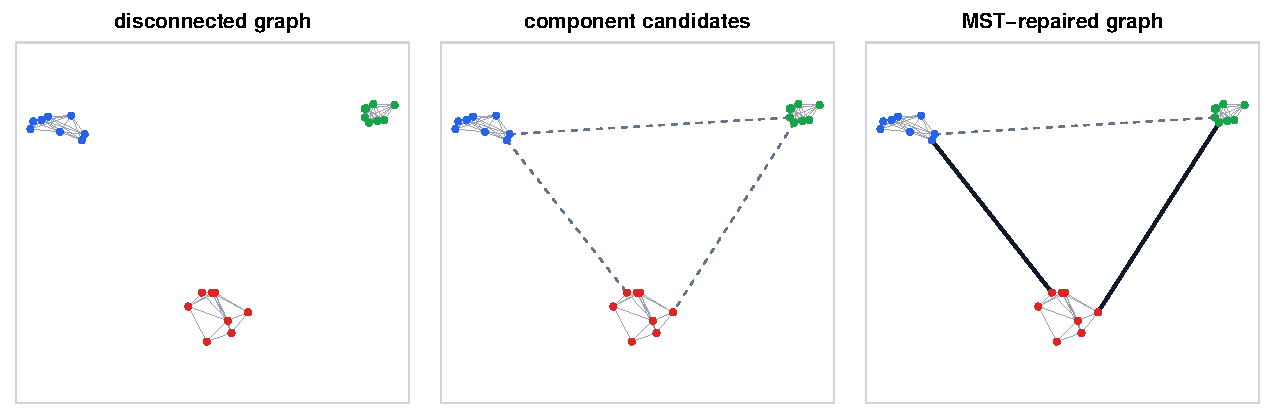
\includegraphics[width=0.95\linewidth]{figures/component_mst_repair_diagram.pdf}
  \caption{Component-MST repair.  Components are first identified, candidate bridge lengths
  are computed between component pairs, and only the component-MST bridge edges are added
  to connect the graph.}
\end{figure}

\texttt{gflow} exposes three repair modes.  \texttt{component.mst} computes exact shortest
intercomponent bridges.  \texttt{component.mst.ann} first tries sparse approximate
nearest-neighbor bridge candidates and falls back to exact repair when needed.
\texttt{global.mst} unions the graph with the full Euclidean MST on all vertices.  The
component-MST method is the most direct choice when the goal is to add the minimum number
of diagnostic bridge edges.

\section{Examples and failure modes}

\subsection{Finite circle examples}

The root-of-unity examples show clean finite support relationships.  Points are
\[
  x_m=(\cos(2\pi m/n),\sin(2\pi m/n)),
  \qquad
  m=0,\ldots,n-1.
\]
For \(n=3,4,5\), \(k=2\).  For \(n=100\), \(k=10\).  All constructions use Euclidean
distances.

\begin{figure}[htbp]
  \centering
  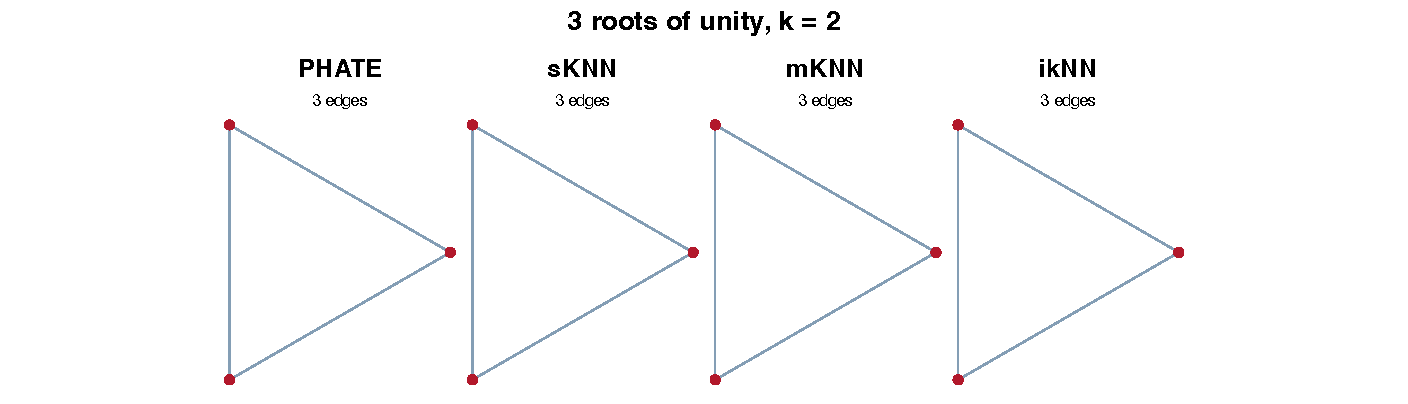
\includegraphics[width=\linewidth]{figures/roots_n3_k2.pdf}
  \caption{Three roots of unity with \(k=2\).  All four constructions produce the complete graph.}
\end{figure}

\begin{figure}[htbp]
  \centering
  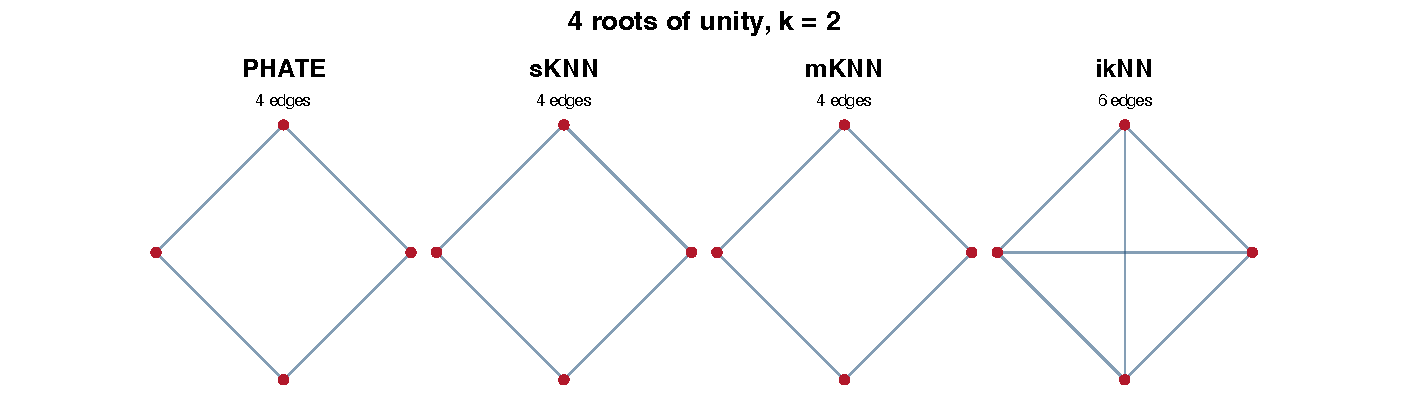
\includegraphics[width=\linewidth]{figures/roots_n4_k2.pdf}
  \caption{Four roots of unity with \(k=2\).  PHATE, sKNN, and mKNN produce the cycle,
  while closed-neighborhood iKNN produces the complete graph.}
\end{figure}

\begin{figure}[htbp]
  \centering
  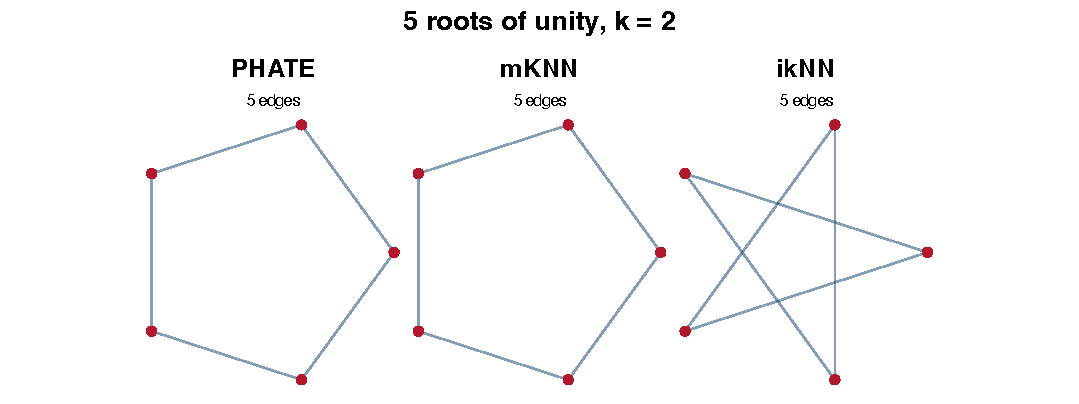
\includegraphics[width=\linewidth]{figures/roots_n5_k2.pdf}
  \caption{Five roots of unity with \(k=2\).  PHATE, sKNN, and mKNN keep adjacent circle
  edges; closed-neighborhood iKNN connects every pair.}
\end{figure}

\begin{figure}[htbp]
  \centering
  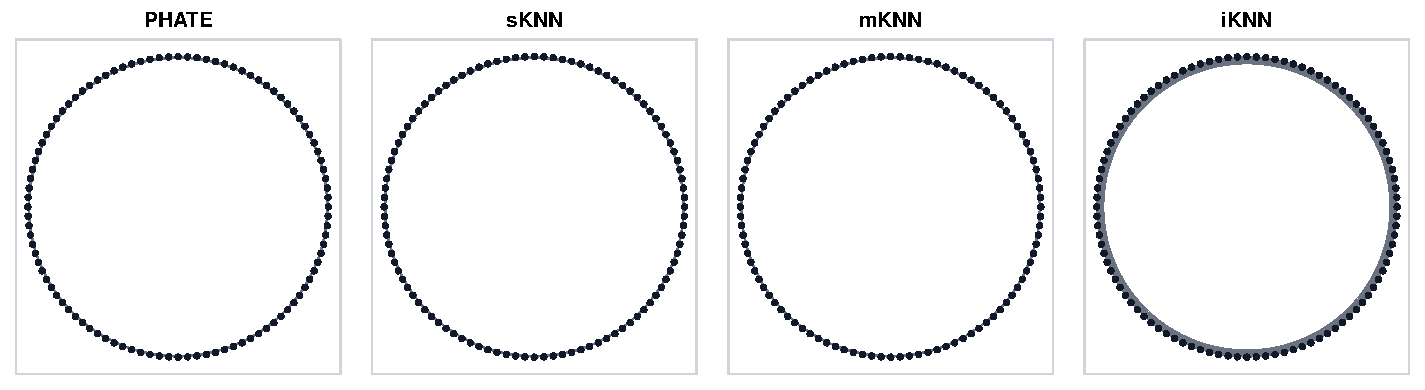
\includegraphics[width=\linewidth]{figures/roots_n100_k10.pdf}
  \caption{One hundred roots of unity with \(k=10\).  PHATE remains close to sKNN, mKNN is
  reciprocal, and iKNN is denser because shared neighborhoods reach farther than direct
  adaptive-radius tests.}
\end{figure}

\subsection{Noisy nonuniform circle and sample Fermat distances}

The noisy-circle examples use a sample Fermat distance as the input \(D\).  Starting from a
base kNN graph in observed Euclidean coordinates, each base edge has cost
\[
  c_{ij}=\|x_i-x_j\|_2^\alpha,
  \qquad \alpha=2,
\]
and the sample Fermat distance is
\[
  d_F(i,j)
  =
  \min_{\gamma:i\leadsto j}
  \sum_{\{u,v\}\in\gamma} c_{uv}.
\]
This powered shortest-path distance penalizes long jumps and can reduce the influence of
noisy ambient shortcuts before the second-stage graph support is constructed.

\begin{figure}[htbp]
  \centering
  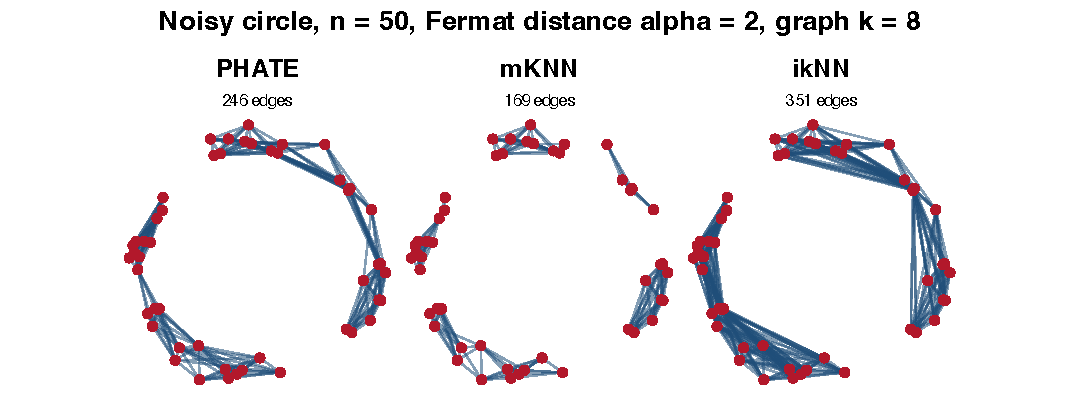
\includegraphics[width=\linewidth]{figures/noisy_circle_fermat_n50_k8.pdf}
  \caption{Noisy circle, \(n=50\), graph \(k=8\), sample Fermat distance with \(\alpha=2\).}
\end{figure}

\begin{figure}[htbp]
  \centering
  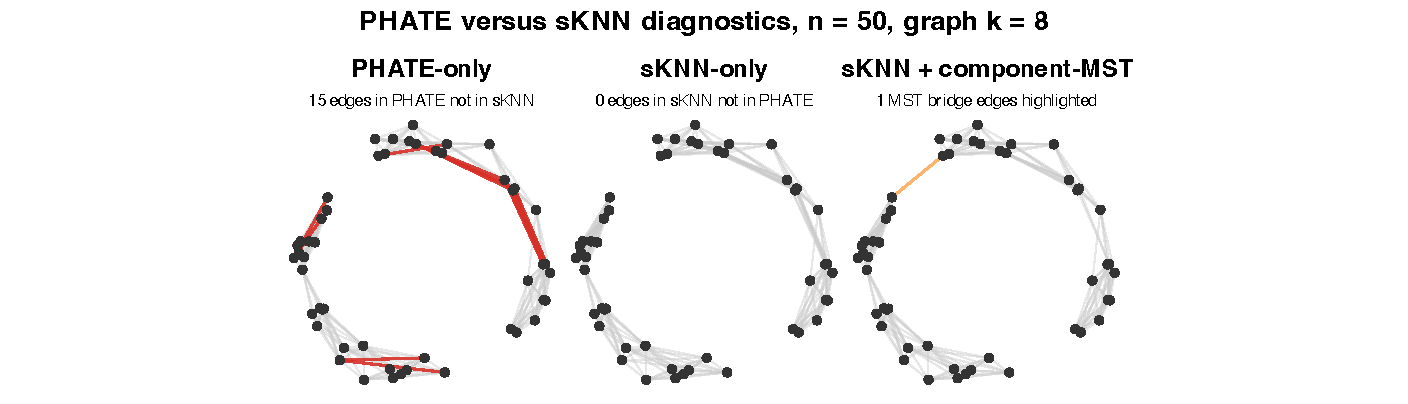
\includegraphics[width=\linewidth]{figures/noisy_circle_fermat_n50_k8_diagnostics.pdf}
  \caption{Noisy circle, \(n=50\), PHATE-versus-sKNN diagnostics and component-MST bridge view.}
\end{figure}

\begin{figure}[htbp]
  \centering
  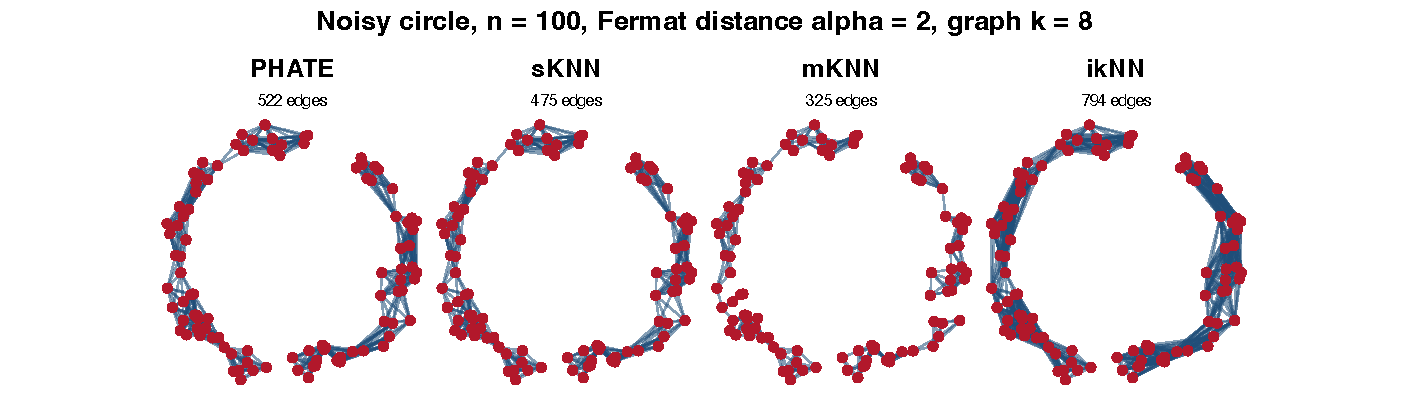
\includegraphics[width=\linewidth]{figures/noisy_circle_fermat_n100_k8.pdf}
  \caption{Noisy circle, \(n=100\), graph \(k=8\), sample Fermat distance with \(\alpha=2\).}
\end{figure}

\begin{figure}[htbp]
  \centering
  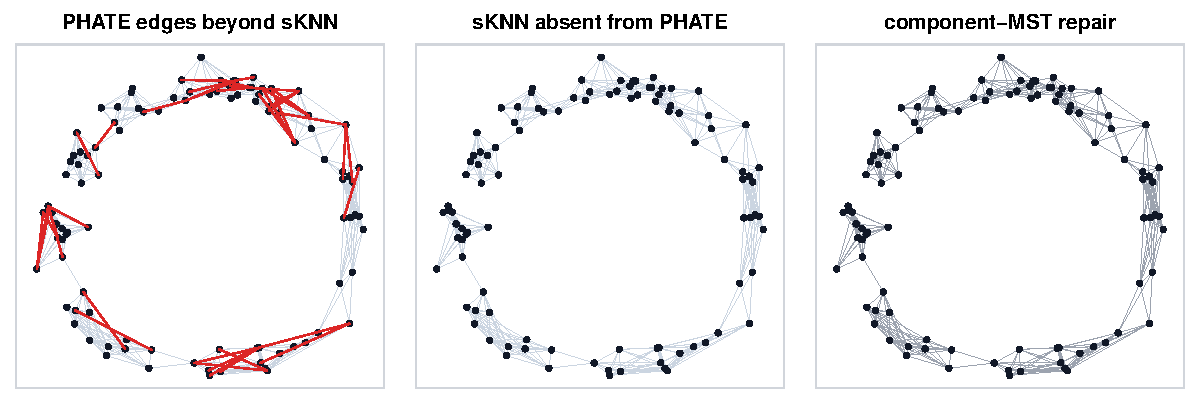
\includegraphics[width=\linewidth]{figures/noisy_circle_fermat_n100_k8_diagnostics.pdf}
  \caption{Noisy circle, \(n=100\), PHATE-versus-sKNN diagnostics and component-MST bridge view.}
\end{figure}

\begin{figure}[htbp]
  \centering
  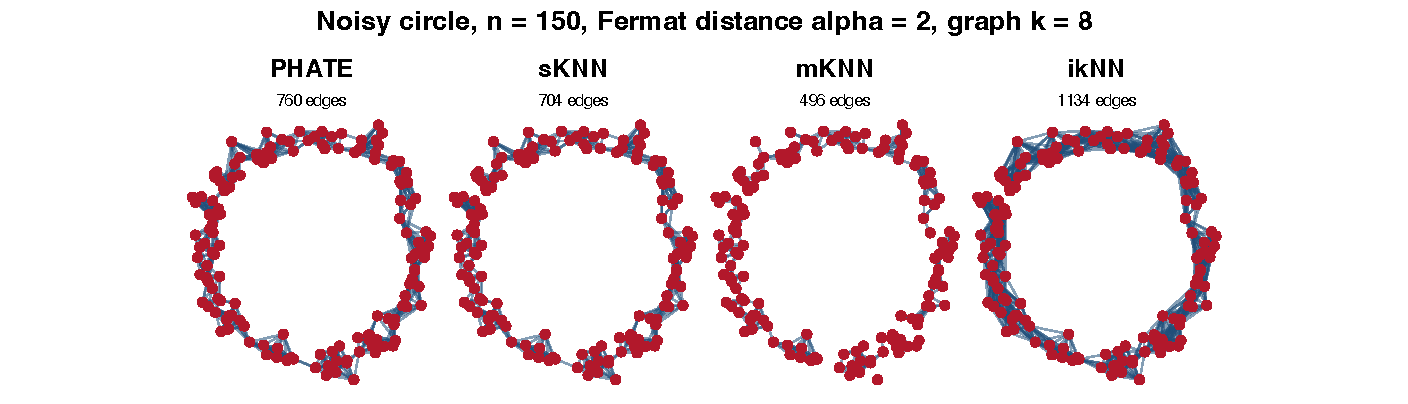
\includegraphics[width=\linewidth]{figures/noisy_circle_fermat_n150_k8.pdf}
  \caption{Noisy circle, \(n=150\), graph \(k=8\), sample Fermat distance with \(\alpha=2\).}
\end{figure}

\begin{figure}[htbp]
  \centering
  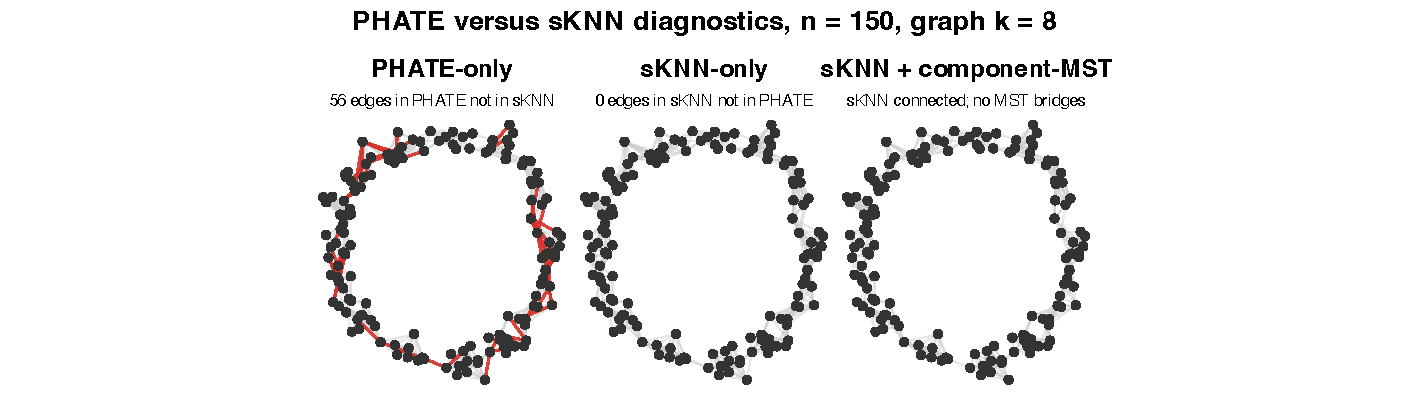
\includegraphics[width=\linewidth]{figures/noisy_circle_fermat_n150_k8_diagnostics.pdf}
  \caption{Noisy circle, \(n=150\), PHATE-versus-sKNN diagnostics and component-MST bridge view.}
\end{figure}

\subsection{Additional 2D stress examples}

Several simple 2D data sets expose distinct failure modes.  A figure eight stresses
self-approach.  Crossing and nearly crossing line segments separate ambient proximity from
branch membership.  A branching tree tests whether a graph preserves arms without creating
shortcuts.  A nonuniform circle shows why global radius rules are density-sensitive.  A
quadratic parameter disk connects the report to the current surface benchmark.

\begin{figure}[htbp]
  \centering
  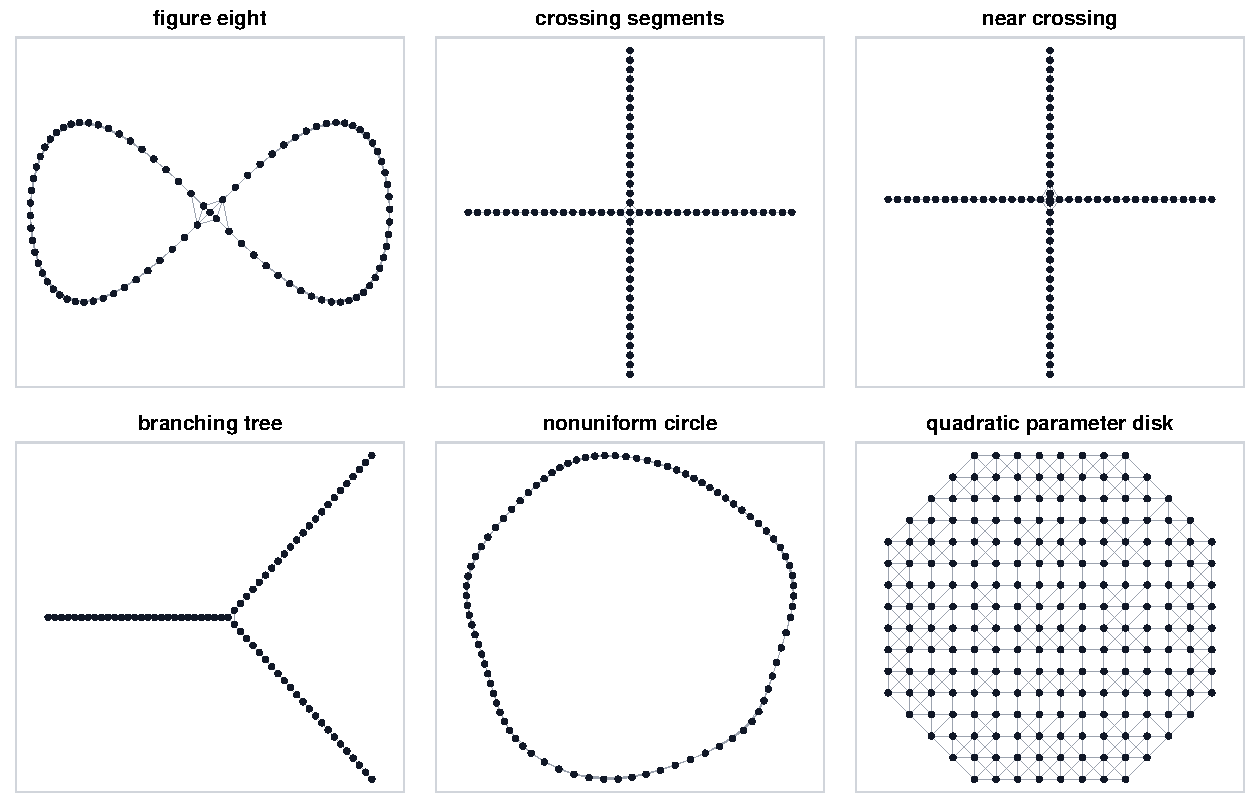
\includegraphics[width=0.95\linewidth]{figures/failure_mode_examples.pdf}
  \caption{Illustrative 2D stress cases for data graph construction.  The displayed edges
  are sKNN supports and are meant as visual examples of possible shortcut and connectivity
  issues, not benchmark conclusions.}
\end{figure}

\subsection{Quadratic graph surfaces}

The current geodesic benchmark focuses on two quadratic graph surfaces over the parameter
disk
\[
  \Omega=\{(u,v)\in\R^2:u^2+v^2\le 1\},
\]
embedded as
\[
  F(u,v)=(u,v,q(u,v)).
\]
The two target surfaces are
\[
  q_{\mathrm{paraboloid}}(u,v)=u^2+v^2,
  \qquad
  q_{\mathrm{saddle}}(u,v)=u^2-v^2.
\]
They are simple enough to support numerical reference geodesics while still curved enough
to reveal distortion in graph shortest-path distances.

\begin{figure}[htbp]
  \centering
  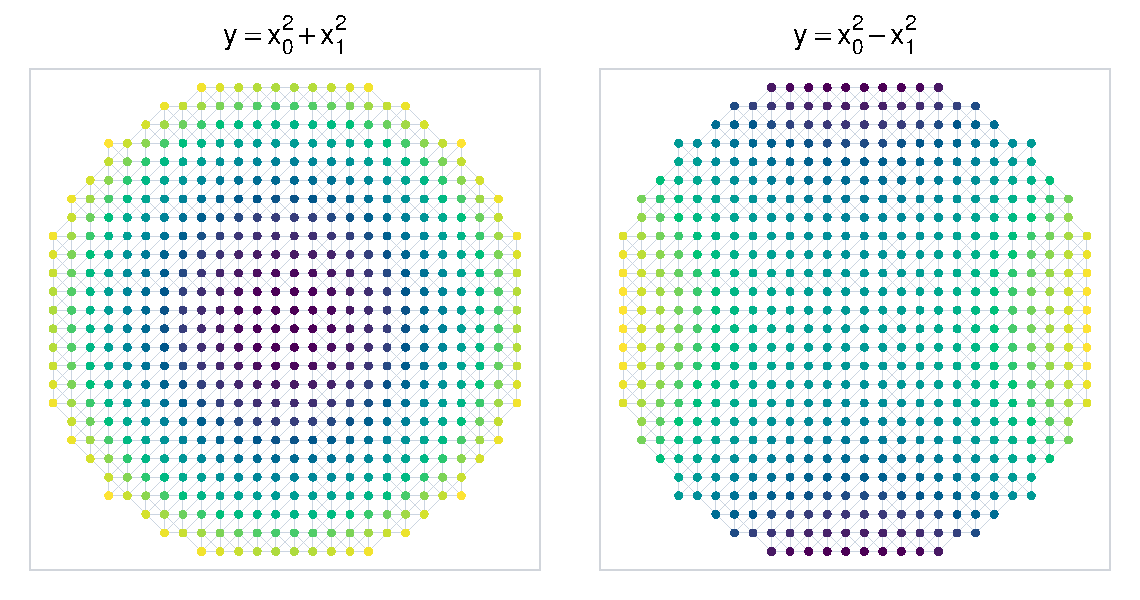
\includegraphics[width=0.88\linewidth]{figures/quadform_surface_examples.pdf}
  \caption{Quadratic graph-surface benchmark examples shown in parameter coordinates, with
  color indicating the graph height \(q(u,v)\).  The benchmark constructs data graphs on
  embedded points \(F(u,v)\) and compares graph shortest paths to reference surface
  geodesics.}
\end{figure}

\section{Evaluation metrics}

Because graph distances can differ from reference distances by a global scale, the benchmark
uses a scale-adjusted comparison.  Given finite distances \(d_G(i,j)\) and a reference
\(d_{\mathrm{ref}}(i,j)\), define
\[
  \alpha^*
  =
  \operatorname*{arg\,min}_{\alpha>0}
  \sum_{i<j}
  \left(\alpha\,d_G(i,j)-d_{\mathrm{ref}}(i,j)\right)^2 .
\]
The relative RMS error is
\[
  \left(
  \frac{
  \sum_{i<j}(\alpha^*d_G(i,j)-d_{\mathrm{ref}}(i,j))^2
  }{
  \sum_{i<j}d_{\mathrm{ref}}(i,j)^2
  }
  \right)^{1/2}.
\]
Additional diagnostics include relative absolute error, distortion quantiles, distance
correlations, component counts, edge counts, bridge counts, and pruning statistics.  These
metrics should always report which graph lifecycle stage and which reference target were
used.

\section{Computational considerations}

Exact pairwise construction is deterministic and simple but costs \(O(n^2)\) memory or time
for the candidate distances.  kNN and adaptive-radius graphs can use nearest-neighbor
search to reduce the candidate set, although exact tie behavior may differ between exact
and approximate search backends.  Fixed-radius graphs are especially sensitive to the cost
of discovering all pairs within \(\eps\) at large \(n\).

Component-MST repair has two costs: finding connected components and finding shortest
intercomponent bridges.  Exact component bridges can be expensive if there are many large
components, while approximate-neighbor bridge candidates are faster but require fallback
logic when they do not connect the component graph.  Local geodesic pruning is currently
the most expensive benchmark stage because it repeatedly computes alternative local
shortest paths while modifying the graph.  That performance issue should be profiled
separately before large pruning sweeps are treated as routine.

\section{Historical perspective}

Isomap made graph shortest paths on neighborhood graphs central to nonlinear dimensionality
reduction.  Its basic estimator builds a kNN or fixed-radius graph, weights local edges by
ambient distance, and uses graph shortest paths as approximate manifold geodesics before
classical multidimensional scaling.  Theoretical work around Isomap and random geometric
graphs clarified the asymptotic promise and the central scale tradeoff: too small a
neighborhood disconnects the graph, too large a neighborhood creates short circuits.

Fixed-radius graphs connect this data-analysis practice to random geometric graphs and
Gilbert's random plane network model.  kNN, symmetric kNN, and mutual kNN became standard
choices in clustering, semi-supervised learning, manifold learning, and spectral methods.
Mutual kNN is often used as a conservative alternative to union kNN when one wants
reciprocal local support.

Adaptive local scaling entered spectral clustering as a way to avoid one global bandwidth.
The same idea appears here as adaptive-radius support: use \(d_{i,(k)}\) as a local scale
and compare \(d_{ij}\) to a function of endpoint scales.  PHATE uses a related adaptive
kernel but then follows an affinity-to-diffusion path rather than a graph-length path.
Shared-nearest-neighbor graphs are another related but distinct lineage: they weight edges
by overlap in neighbor lists, as in the Jarvis-Patrick idea and modern single-cell SNN
workflows.  \texttt{gflow}'s iKNN support also uses neighborhood intersections, but its edge
predicate and native detour length should not be confused with Jaccard-style SNN weights.

Pruning belongs to a broader geometric sparsification tradition.  Graph spanners ask for
sparser subgraphs that approximately preserve distances.  Local geodesic pruning borrows
that intuition, but in this report it remains an empirical data-graph procedure: remove
locally replaceable edges and then measure whether geodesic reconstruction improves.  MST
repair has a different role.  It is a connectivity scaffold, grounded in classical minimum
spanning tree algorithms, and should be reported as an explicit intervention rather than a
native neighborhood relation.

\section*{References}

\begin{enumerate}[leftmargin=2em]
  \item J. B. Tenenbaum, V. de Silva, and J. C. Langford. ``A global geometric
  framework for nonlinear dimensionality reduction.'' \emph{Science} 290(5500),
  2319--2323, 2000.  Isomap introduced kNN or radius graph shortest paths as
  manifold-geodesic estimates for nonlinear embedding.

  \item D. L. Donoho and C. Grimes. ``Hessian eigenmaps: locally linear embedding
  techniques for high-dimensional data.'' \emph{PNAS} 100(10), 5591--5596, 2003.
  This is one representative of the broader manifold-learning context in which local
  neighborhoods approximate intrinsic geometry.

  \item E. N. Gilbert. ``Random plane networks.'' \emph{Journal of the Society for
  Industrial and Applied Mathematics} 9(4), 533--543, 1961.  This is a classical
  origin of random geometric graph models.

  \item M. Penrose. \emph{Random Geometric Graphs}. Oxford University Press, 2003.
  This monograph develops the probability theory of radius-based random geometric graphs.

  \item L. Zelnik-Manor and P. Perona. ``Self-tuning spectral clustering.'' In
  \emph{Advances in Neural Information Processing Systems} 17, 2004.  This paper
  popularized local-scale kernels for spectral clustering.

  \item M. Maier, U. von Luxburg, and M. Hein. ``Influence of graph construction on
  graph-based clustering measures.'' In \emph{Advances in Neural Information Processing
  Systems} 22, 2009.  This work discusses how choices such as symmetric and mutual kNN
  affect graph-based clustering behavior.

  \item R. A. Jarvis and E. A. Patrick. ``Clustering using a similarity measure based on
  shared near neighbors.'' \emph{IEEE Transactions on Computers} C-22(11),
  1025--1034, 1973.  This is a classical shared-nearest-neighbor reference.

  \item K. R. Moon, D. van Dijk, Z. Wang, S. Gigante, D. B. Burkhardt, W. S. Chen,
  K. Yim, A. van den Elzen, M. J. Hirn, R. R. Coifman, N. B. Ivanova, G. Wolf, and
  S. Krishnaswamy. ``Visualizing structure and transitions in high-dimensional
  biological data.'' \emph{Nature Biotechnology} 37, 1482--1492, 2019.  This is the
  PHATE paper.

  \item I. Althoefer, G. Das, D. Dobkin, D. Joseph, and J. Soares. ``On sparse spanners
  of weighted graphs.'' \emph{Discrete \& Computational Geometry} 9, 81--100, 1993.
  This is a foundational graph-spanner reference for distance-preserving sparsification.

  \item G. Narasimhan and M. Smid. \emph{Geometric Spanner Networks}. Cambridge
  University Press, 2007.  This book surveys geometric spanner theory.

  \item J. B. Kruskal. ``On the shortest spanning subtree of a graph and the traveling
  salesman problem.'' \emph{Proceedings of the American Mathematical Society} 7(1),
  48--50, 1956.

  \item R. C. Prim. ``Shortest connection networks and some generalizations.''
  \emph{Bell System Technical Journal} 36(6), 1389--1401, 1957.

  \item D. Groisman, M. Jonckheere, and F. Sapienza. ``Nonhomogeneous Euclidean
  first-passage percolation and distance learning.'' arXiv:1810.09398, 2018.
  This work is part of the Fermat-distance literature.

  \item N. Garcia Trillos, M. Gerlach, M. Hein, and D. Slepcev. ``Fermat distances:
  metric approximation, spectral convergence, and clustering algorithms.''
  \emph{Journal of Machine Learning Research} 25, 2024.
\end{enumerate}

\end{document}
